\begin{frame}{simple-module}{Modul f�r \host}
 \begin{description}[Makefile]
  \item[Code]     \cod{scr/simple-module.c}
%  \item[Makefile] \cod{src/Makefile} von linux Makefile aufgerufen
  \item[Script]   \cod{tools/module.sh} f�r einfachen Aufruf
  \item[Makefile] \cod{src/Makefile} f�r mehr Module
  \item[Test]
      \begin{itemize}
	\item \cod{dmesg -w}
        \item \cod{sudo insmod simple-module.ko} wir sind in \cod{src} 
	\item \cod{lsmod | grep simple} ist installiert
	\item \cod{sudo rmmod simple-module} deinstalliert
	\item Der File \url{proc/modules}
      \end{itemize}
 \end{description}
\end{frame}

\begin{frame}{simple-module}{Modul f�r \targetS}
 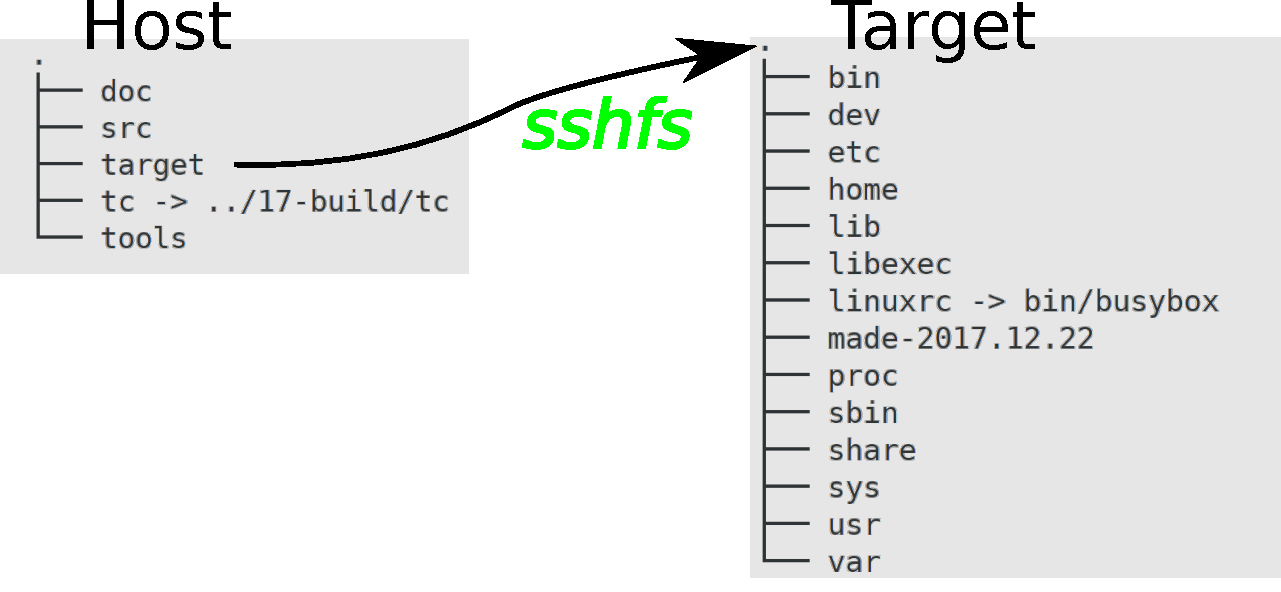
\includegraphics[width=\textwidth]{host-target.pdf}
 \begin{textblock}{100}(10,60)
  \begin{itemize}
   \item \cod{src/Makefile} anpassen
   \item \cod{cp src/{\em module} target/home/root}
   
  \end{itemize}
 \end{textblock}
\end{frame}


